% This work is made available under the terms of the 
% Creative Commons Attribution-ShareAlike 4.0 license,
% http://creativecommons.org/licenses/by-sa/4.0/.

\documentclass[a4paper]{book}

\usepackage{wrapfig}
\usepackage{graphicx}
\usepackage{hyperref}
\usepackage{multirow}
\usepackage{scalefnt}
\usepackage{tikz}

% watermark -- for draft stage
%\usepackage[firstpage]{draftwatermark}
%\SetWatermarkLightness{0.9}
%\SetWatermarkScale{5}

% Copyright (c) 2009 by the University of Waikato, Hamilton, NZ. 
% This work is made available under the terms of the 
% Creative Commons Attribution-ShareAlike 4.0 license,
% http://creativecommons.org/licenses/by-sa/4.0/.
%
% Version: $Revision: 6032 $

\newenvironment{tight_itemize}{
\begin{itemize}
  \setlength{\itemsep}{1pt}
  \setlength{\parskip}{0pt}
  \setlength{\parsep}{0pt}}{\end{itemize}
}

\newenvironment{tight_enumerate}{
\begin{enumerate}
  \setlength{\itemsep}{1pt}
  \setlength{\parskip}{0pt}
  \setlength{\parsep}{0pt}}{\end{enumerate}
}

% if you just need a simple heading
% Usage:
%   \heading{the text of the heading}
\newcommand{\heading}[1]{
  \vspace{0.3cm} \noindent \textbf{#1} \newline
}

\newcommand{\icon}[1]{\tikz[baseline=-3pt]\node[inner sep=0pt,outer sep=0pt]{\includegraphics[height=1.1em]{#1}};}


\title{
  \textbf{ADAMS} \\
  {\Large \textbf{A}dvanced \textbf{D}ata mining \textbf{A}nd \textbf{M}achine
  learning \textbf{S}ystem} \\
  {\Large Module: adams-spectral-2dim-core} \\
  \vspace{1cm}
  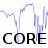
\includegraphics[width=2cm]{images/spectral-2dim-core-module.png} \\
}
\author{
  Peter Reutemann
}

\setcounter{secnumdepth}{3}
\setcounter{tocdepth}{3}

\begin{document}

\begin{titlepage}
\maketitle

\thispagestyle{empty}
\center
\begin{table}[b]
	\begin{tabular}{c l l}
		\parbox[c][2cm]{2cm}{\copyright 2017-2021} &
		\parbox[c][2cm]{5cm}{
\includegraphics[width=5cm]{images/coat_of_arms.pdf}} \\
	\end{tabular}
	
\includegraphics[width=12cm]{images/cc.png} \\
\end{table}

\end{titlepage}

\tableofcontents
\listoffigures
%\listoftables

%%%%%%%%%%%%%%%%%%%%%%%%%%%%%%%%%%%
\chapter{Introduction}
The \textit{adams-spectral-2dim-core} module offers a comprehensive suite
of tools and data processing of two-dimensional spectra, such as generted from
near-infrared\cite{nir}, mid-infrared\cite{mir} and X-ray fluorescence\cite{xrf}
instruments.

%%%%%%%%%%%%%%%%%%%%%%%%%%%%%%%%%%%
\chapter{Flow}
The following conversions are available:
\begin{tight_itemize}
  \item \textit{MultiSpectrumToSpectra} -- turns a single multi-spectrum
  into an array of regular spectra.
  \item \textit{ReportToSampleData} -- converts a simple report into
  a sample data object.
  \item \textit{SampleDataArrayToMap} -- converts a sample data array to a map, using the sample ID as key.
  \item \textit{SpectraToMultiSpectrum} -- turns an array of spectra
  into a single multi-spectrum.
  \item \textit{SpectrumToArray} -- turns a spectrum into a float array
  (either wave numbers or amplitudes).
  \item \textit{SpectrumToJson} -- turns a spectrum into a JSON object.
  \item \textit{SpectrumToSpreadSheet} -- turns a spectrum into a spreadsheet
  with two columns: wave numbers and amplitudes.
  \item \textit{SpreadSheetColumnsToSampleData} -- generates sample data objects from the columns in a spreadsheet.
  \item \textit{SpreadSheetColumnsToSpectra} -- generates spectra from the columns in a spreadsheet.
  \item \textit{SpreadSheetRowsToSampleData} -- generates sample data objects from the rows in a spreadsheet.
  \item \textit{SpreadSheetRowsToSpectra} -- generates spectra from the rows in a spreadsheet.
  \item \textit{SpreadSheetToSpectrum} -- generates a spectrum from a spreadsheet
  with two columns containing the wave numbers and amplitudes.
  \item \textit{WekaPredictionContainerToEvaluationContainer} -- turns the
  prediction container into an evaluation container.
\end{tight_itemize}
The following sources are available:
\begin{tight_itemize}
  \item \textit{InstrumentSupplier} -- returns all instrument names from the
  database.
  \item \textit{NewSpectrum} -- creates an empty spectrum.
  \item \textit{SpectrumIdSupplier} -- outputs database or sample IDs from spectra
  stored in the database.
  \item \textit{OrphanedSampleDataIdSupplier} -- allows the retrieval of sample
  IDs of sample data that have no spectra associated.
  \item \textit{SQLSpectrumIdSupplier} -- outputs IDs (integer or string)
  generated from a SQL query.
\end{tight_itemize}
The following transformers are available:
\begin{tight_itemize}
  \item \textit{Cleaner} -- cleans a Weka dataset with a specific cleaner
  and performs checks on single Instance objects.
  \item \textit{DeleteDbSampleDataValue} -- removes the specified fields
  from the sampledata table for a specific sample ID.
  \item \textit{DeleteSampleDataValue} -- removes the specified fields
  from the sample data passing through.
  \item \textit{DeleteSampleDataValueByExpression} -- deletes a specific
  field from sample data if the boolean expression evaluates to true.
  \item \textit{DeleteSpectrum} -- removes a spectrum, identified by
  database or sample ID, from the database.
  \item \textit{Evaluator} -- trains an evaluator on a Weka dataset and
  applies the evaluator on single Weka Instance objects.
  \item \textit{GetSampleDataValue} -- retrieves a single value from a
  sample data object.
  \item \textit{GetSpectrumAmplitude} -- retrieves the amplitude of the
  specified wave number.
  \item \textit{InstanceGenerator} -- turns a spectrum into a Weka Instance.
  \item \textit{InstanceToSpectrum} -- turns a Weka Instance into a spectrum.
  \item \textit{MultiSpectrumAdd} -- adds a spectrum obtained from storage or
  callable actor to the multi-spectrum passing through.
  \item \textit{MultiSpectrumFilter} -- applies a filter to a multi-spectrum.
  \item \textit{MultiSpectrumOutlierDetector} -- applies outlier detectors
  to multi-spectra.
  \item \textit{MultiSpectrumRemove} -- removes spectra from a multi-spectrum
  that match expressions on sample ID, type or format.
  \item \textit{MultiSpectrumReportFilter} -- filters the reports of a
  multi-spectrum.
  \item \textit{PostProcessor} -- allows the post-processing of Weka Instances.
  \item \textit{SampleDataDbReader} -- reads sample data from the database.
  \item \textit{SampleDataDbWriter} -- writes sample data to the database.
  \item \textit{SampleDataFileReader} -- loads sample data from disk.
  \item \textit{SampleDataFileWriter} -- writes sample data to disk.
  \item \textit{SampleDataValueDbWriter} -- writes specific sample data fields
  to the database.
  \item \textit{SetSampleDataValue} -- sets the value for the specified
  sample data field.
  \item \textit{SetSpectrumAmplitude} -- set the amplitude of the
  specified wave number or adds a new spectrum point altogether.
  \item \textit{SpectrumAppend} -- appens the incoming spectrum to the one
  in storage (latter doesn't have to be present).
  \item \textit{SpectrumDbReader} -- loads a spectrum from the database.
  \item \textit{SpectrumDbWriter} -- writes a spectrum to the database.
  \item \textit{SpectrumDiff} -- calculates the difference between the
  two spectra received as array and outputs the difference as spectrum.
  \item \textit{SpectrumFeatureGenerator} -- for generating features from
  a spectrum.
  \item \textit{SpectrumFileReader} -- loads a spectrum from disk.
  \item \textit{SpectrumFileWriter} -- writes a spectrum to disk.
  \item \textit{SpectrumFilter} -- applies a filter to the spectrum passing through.
  \item \textit{SpectrumInfo} -- outputs information about a spectrum.
  \item \textit{SpectrumMinMax} -- for keeping track of min/max amplitudes per
  wave number (and outputs these).
\end{tight_itemize}
The following sinks are available:
\begin{tight_itemize}
  \item \textit{SampleDataDisplay} -- displays one or more sample data reports.
  \item \textit{SpectrumDisplay} -- displays one or more spectra.
  \item \textit{SpectrumImageWriter} -- writes a spectrum as an image.
\end{tight_itemize}

%%%%%%%%%%%%%%%%%%%%%%%%%%%%%%%%%%%
\chapter{Visualization}
The \textit{Spectrum Explorer} (see Figure \ref{spectrum_explorer}) allows you
to load spectra of various types from disk or database for visual inspection,
as well as processing via filters. PCA and PLS analysis are possible as well.
The spectra can be exported any time as well.
Actions in the GUI can be recorded as scripts and the replayed easily.

\begin{figure}[htb]
  \centering
  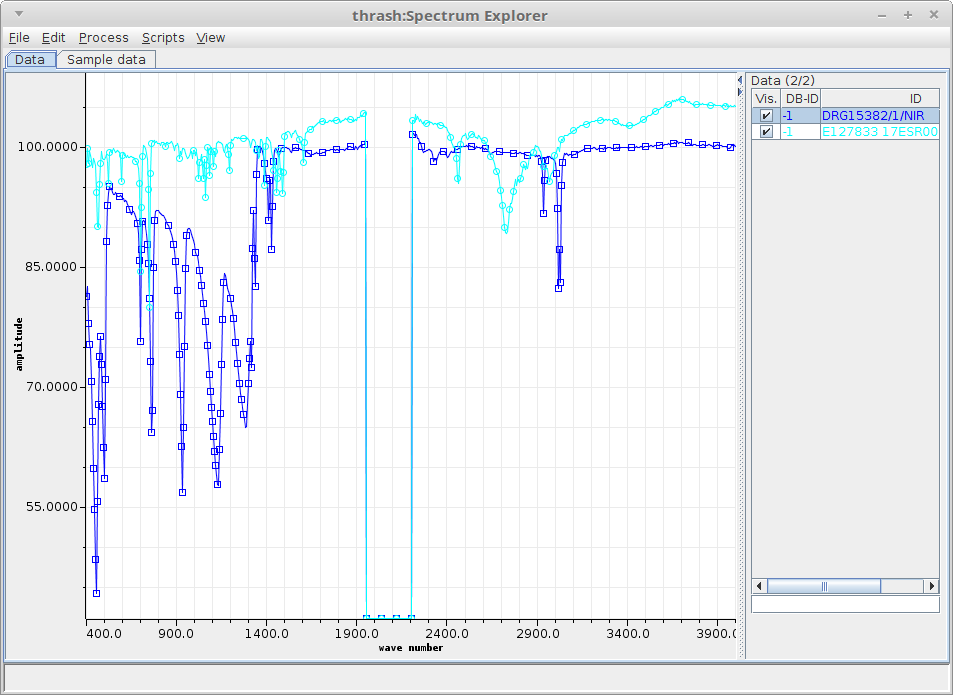
\includegraphics[width=12.0cm]{images/spectrum_explorer.png}
  \caption{Spectrum Explorer}
  \label{spectrum_explorer}
\end{figure}

%%%%%%%%%%%%%%%%%%%%%%%%%%%%%%%%%%%
\chapter{Maintenance}
The following maintenance tools are available:
\begin{tight_itemize}
  \item \textit{Delete spectra} -- allows removal of spectra from the database.
  \item \textit{Delete sample data} -- interface for deleting specified sample data values
  in selected spectra.
  \item \textit{List sample data} -- interface for listing all sample data values
  in selected spectra.
  \item \textit{Update sample data} -- interface for updating sample data values
  in selected spectra.
\end{tight_itemize}

%%%%%%%%%%%%%%%%%%%%%%%%%%%%%%%%%%%
% Copyright (c) 2009-2012 by the University of Waikato, Hamilton, NZ. 
% This work is made available under the terms of the 
% Creative Commons Attribution-ShareAlike 4.0 license,
% http://creativecommons.org/licenses/by-sa/4.0/.
%
% Version: $Revision: 6032 $

\begin{thebibliography}{999}
  % to make the bibliography appear in the TOC
  \addcontentsline{toc}{chapter}{Bibliography}

  % references
  \bibitem{adams}
    \textit{ADAMS} -- Advanced Data mining and Machine learning System \\
    \url{https://adams.cms.waikato.ac.nz/}{}

  \bibitem{nir}
    \textit{NIR} -- Near-infrared spectroscopy \\
    \url{https://en.wikipedia.org/wiki/Near-infrared_spectroscopy}{}

  \bibitem{mir}
    \textit{MIR} -- Near-infrared spectroscopy \\
    \url{https://en.wikipedia.org/wiki/Mid-infrared}{}

  \bibitem{xrf}
    \textit{XRF} -- X-ray fluorescence \\
    \url{https://en.wikipedia.org/wiki/X-ray_fluorescence}{}

\end{thebibliography}


\end{document}
